\documentclass[a4paper]{article}\usepackage[]{graphicx}\usepackage[]{color}
%% maxwidth is the original width if it is less than linewidth
%% otherwise use linewidth (to make sure the graphics do not exceed the margin)
\makeatletter
\def\maxwidth{ %
  \ifdim\Gin@nat@width>\linewidth
    \linewidth
  \else
    \Gin@nat@width
  \fi
}
\makeatother

\definecolor{fgcolor}{rgb}{0.345, 0.345, 0.345}
\newcommand{\hlnum}[1]{\textcolor[rgb]{0.686,0.059,0.569}{#1}}%
\newcommand{\hlstr}[1]{\textcolor[rgb]{0.192,0.494,0.8}{#1}}%
\newcommand{\hlcom}[1]{\textcolor[rgb]{0.678,0.584,0.686}{\textit{#1}}}%
\newcommand{\hlopt}[1]{\textcolor[rgb]{0,0,0}{#1}}%
\newcommand{\hlstd}[1]{\textcolor[rgb]{0.345,0.345,0.345}{#1}}%
\newcommand{\hlkwa}[1]{\textcolor[rgb]{0.161,0.373,0.58}{\textbf{#1}}}%
\newcommand{\hlkwb}[1]{\textcolor[rgb]{0.69,0.353,0.396}{#1}}%
\newcommand{\hlkwc}[1]{\textcolor[rgb]{0.333,0.667,0.333}{#1}}%
\newcommand{\hlkwd}[1]{\textcolor[rgb]{0.737,0.353,0.396}{\textbf{#1}}}%

\usepackage{framed}
\makeatletter
\newenvironment{kframe}{%
 \def\at@end@of@kframe{}%
 \ifinner\ifhmode%
  \def\at@end@of@kframe{\end{minipage}}%
  \begin{minipage}{\columnwidth}%
 \fi\fi%
 \def\FrameCommand##1{\hskip\@totalleftmargin \hskip-\fboxsep
 \colorbox{shadecolor}{##1}\hskip-\fboxsep
     % There is no \\@totalrightmargin, so:
     \hskip-\linewidth \hskip-\@totalleftmargin \hskip\columnwidth}%
 \MakeFramed {\advance\hsize-\width
   \@totalleftmargin\z@ \linewidth\hsize
   \@setminipage}}%
 {\par\unskip\endMakeFramed%
 \at@end@of@kframe}
\makeatother

\definecolor{shadecolor}{rgb}{.97, .97, .97}
\definecolor{messagecolor}{rgb}{0, 0, 0}
\definecolor{warningcolor}{rgb}{1, 0, 1}
\definecolor{errorcolor}{rgb}{1, 0, 0}
\newenvironment{knitrout}{}{} % an empty environment to be redefined in TeX

\usepackage{alltt}
\usepackage{a4wide}
\usepackage[authoryear]{natbib}
\usepackage{amsmath}

%\SweaveOpts{engine=R, eps=FALSE, keep.source = FALSE}
%\VignetteIndexEntry{Simple example analyses}
%\VignetteDepends{QPress}
%\VignettePackage{QPress}
\IfFileExists{upquote.sty}{\usepackage{upquote}}{}
\begin{document}
\SweaveOpts{concordance=TRUE}

\title{Mesocosm Examples}
\date{2013}
\author{\textbf{Jessica Melbourne-Thomas} \\
Australian Antarctic Division\\
Antarctic Climate \& Ecosystems CRC\\
\and \textbf{Ben Raymond} \\
Australian Antarctic Division\\
Antarctic Climate \& Ecosystems CRC\\
\and \textbf{Andrew Constable} \\
Australian Antarctic Division\\
Antarctic Climate \& Ecosystems CRC\\
\and \textbf{Simon Wotherspoon} \\
Australian Antarctic Division\\
Institute for Marine and Antarctic Studies\\
University of Tasmania}
\maketitle

\begin{abstract}
The \textbf{QPress} package provides facilities for modelling the qualitative
impact of a press perturbation upon a network model. This document illustrates
the comparison of alternative models in terms of their responses to perturbation.
Two examples are provided for experimental mesocosms in (I) a lake environment
\citep{Hulot2000}, and (II) Antarctica (Davidson et al. unpublished).
\end{abstract}

\section{Introduction}
\label{sec:introduction}
An experimental mesocosm is an ecological tool that enables the experimenter to
asses assemblage-level responses to environmental change. Mesocosm experiments
are performed in the `natural environment' rather than in a laboratory, but in
an enclosure that is small enough that key variables can be directly controlled.
Because the responses of component species to perturbation can be observed
directly in a mesocosm setting, the results from such studies lend themselves to
analysis using qualitative network modelling. In particular, these analyses can
be used to make inferences regarding the trophic and competitive interactions
that drive assemblage-level responses to perturbation in a mesocosm setting and
potentially more broadly.

In this document we use the \textbf{QPress} package to analyse two sets of
models corresponding to two separate mesocosm experiments. Example I is for
experimental mesocosms in a lake in France that were subjected to high and low
nutrient treatments \citep{Hulot2000}. Example II examines the effects of
elevated concentrations of $\mathrm{CO}_2$ on the Southern Ocean microbial loop,
studied in environmentally controlled tanks (referred to as `minicosms' by the
authors) in Antarctica (Davidson et al. unpublished).

\section{Example I: Lake mesocosm}
\cite{Hulot2000} describe an eight-variable lake mesocosm model comprising
phosphorous, three algal groups, two size-classes of herbivores, invertebrate
carnivores and carnivorous fish (Figure~\ref{fig:Lake}). Unambiguous,
directional responses of model components to increased phosphorous observed in the
mesocosm experiment were increases in each of: phosphorous (Phos), large herbivores
(Herb2), fish (Carn2) and periphyton (AlgP). \cite{JMT2012} compare the ability
of Hulot et al.'s original model (Figure~\ref{fig:Lake}a) and a variant of the
model with one edge added and one edge deleted (Figure~\ref{fig:Lake}b) to
reproduce these changes in response to a positive perturbation to phosphorous.
Specifically, the variant of the original model (model (b) in
Figure~\ref{fig:Lake}b) includes a self-limitation effect for invertebrate
carnivores, and the predator-prey edge from fish to invertebrate carnivores has
been deleted.
\vspace{1cm}

\begin{figure}[ht]
  \centering
  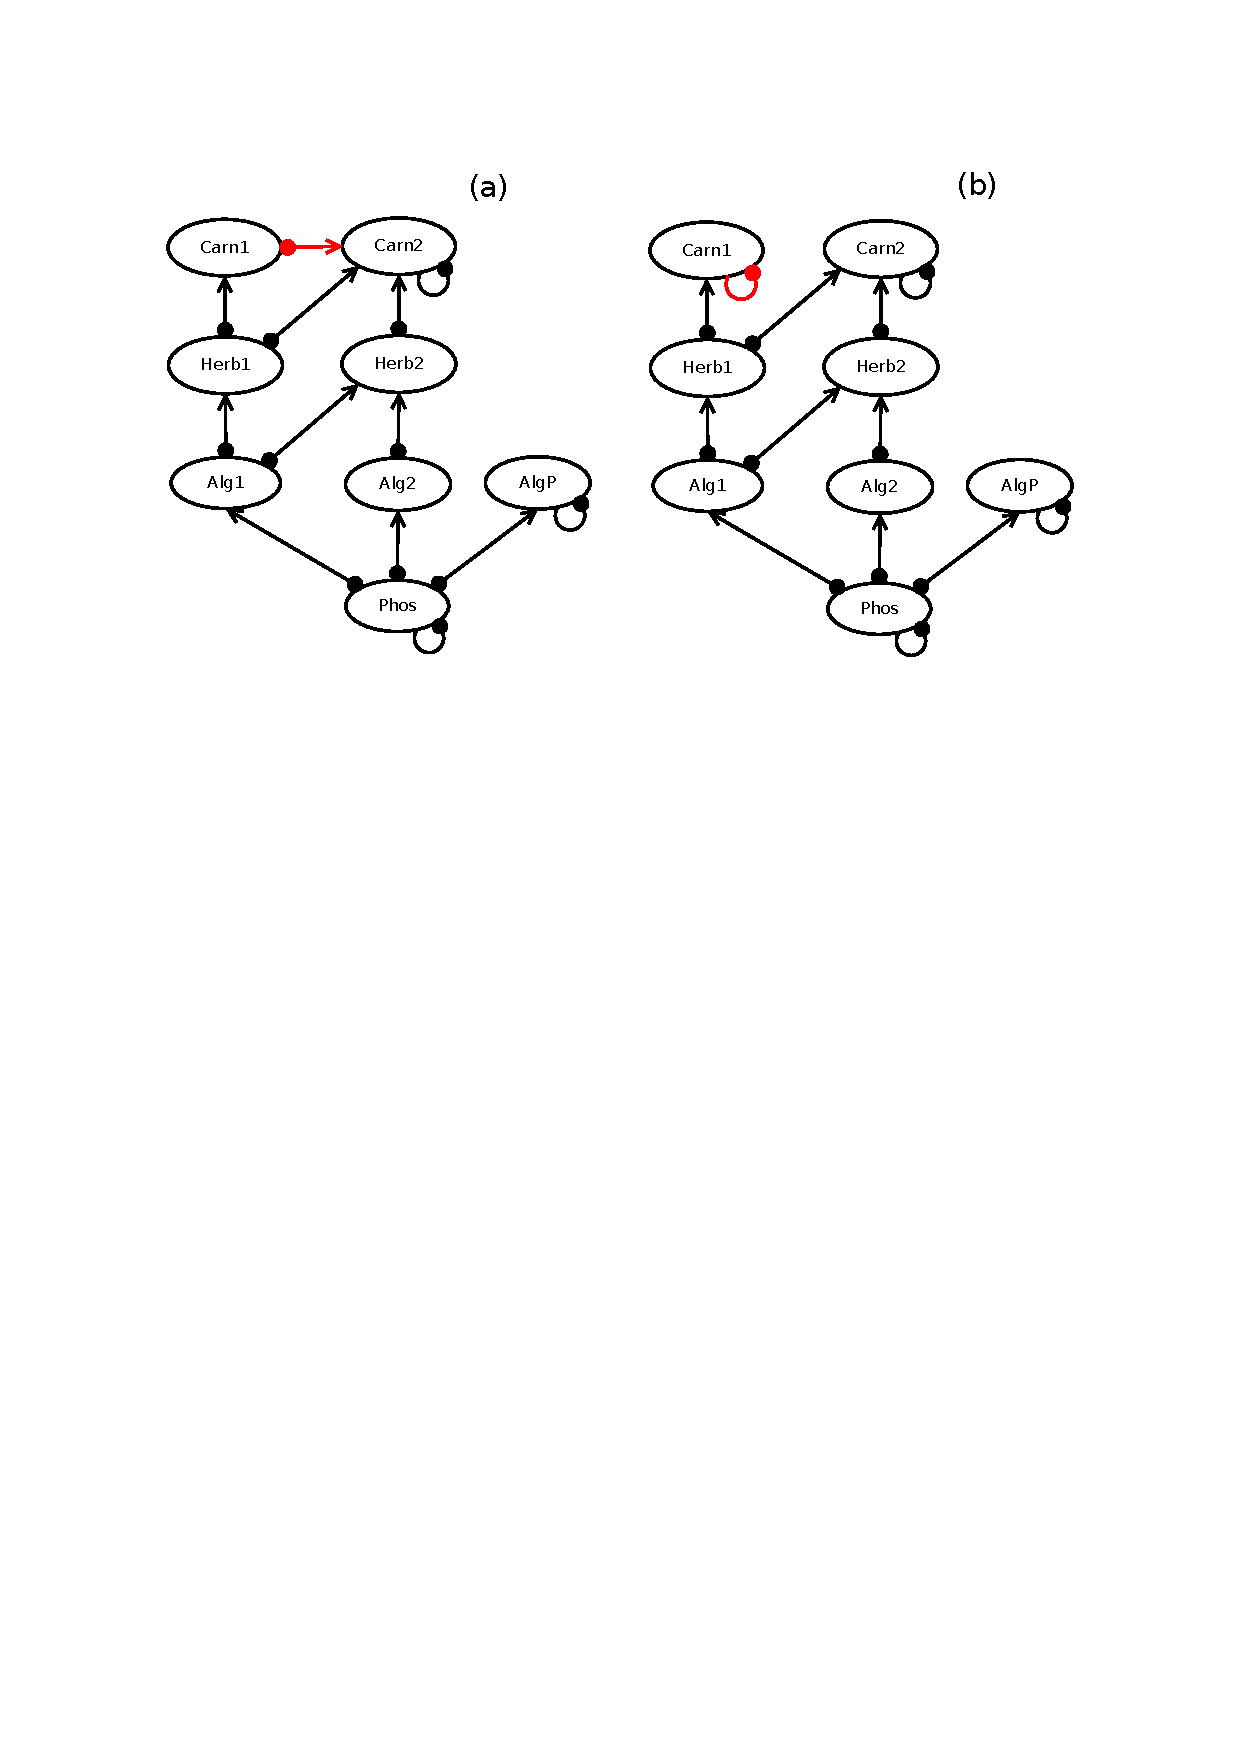
\includegraphics{Lake.pdf}
  \caption{Two versions of the eight-variable lake mesocosm model analyzed by
  \cite{JMT2012} and \cite{Hosack2008}, and originally presented by
  \cite{Hulot2000}. Abbreviations are: Alg1, edible algae; Alg2,
  protected algae; AlgP, periphyton; Carn1,  invertebrate carnivores; Carn2,
  fish; Herb1, small herbivores; Herb2, large herbivores; Phos, phosphorus.}
  \label{fig:Lake}
\end{figure}
\vspace{1cm}

The models shown in Figure~\ref{fig:Lake} were created using Dia and so are
read using \texttt{model.dia}. Here we assign the two model objects to
\texttt{lake.a} and \texttt{lake.b}.
\begin{knitrout}
\definecolor{shadecolor}{rgb}{0.969, 0.969, 0.969}\color{fgcolor}\begin{kframe}
\begin{alltt}
\hlkwd{library}\hlstd{(QPress)}
\hlstd{lake.a} \hlkwb{<-} \hlkwd{model.dia}\hlstd{(}\hlstr{"Lake-a.dia"}\hlstd{)}
\hlstd{lake.b} \hlkwb{<-} \hlkwd{model.dia}\hlstd{(}\hlstr{"Lake-b.dia"}\hlstd{)}
\end{alltt}
\end{kframe}
\end{knitrout}
We then simulate for model (a) and use \texttt{impact.barplot} to view
simulation outcomes corresponding with observations from the mesocosm
experiment (Figure~\ref{fig:Selector1}).

@
\begin{knitrout}
\definecolor{shadecolor}{rgb}{0.969, 0.969, 0.969}\color{fgcolor}\begin{kframe}
\begin{alltt}
\hlstd{simlake.a} \hlkwb{<-} \hlkwd{system.simulate}\hlstd{(}\hlnum{1000}\hlstd{,lake.a)}
\hlkwd{impact.barplot}\hlstd{(simlake.a)}
\end{alltt}
\end{kframe}
\end{knitrout}
Doing the same for model (b) gives Figure~\ref{fig:Perturb1}.

\begin{figure}[ht]
  \centering
  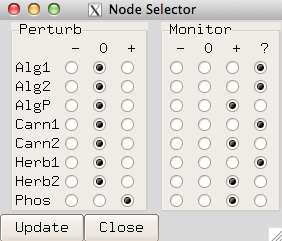
\includegraphics[width=0.3\textwidth]{Lake-selector.png}
  \caption{Node selector for the lake mesocosm example.}
  \label{fig:Selector1}
\end{figure}

\begin{figure}[ht]
  \centering
\begin{knitrout}
\definecolor{shadecolor}{rgb}{0.969, 0.969, 0.969}\color{fgcolor}
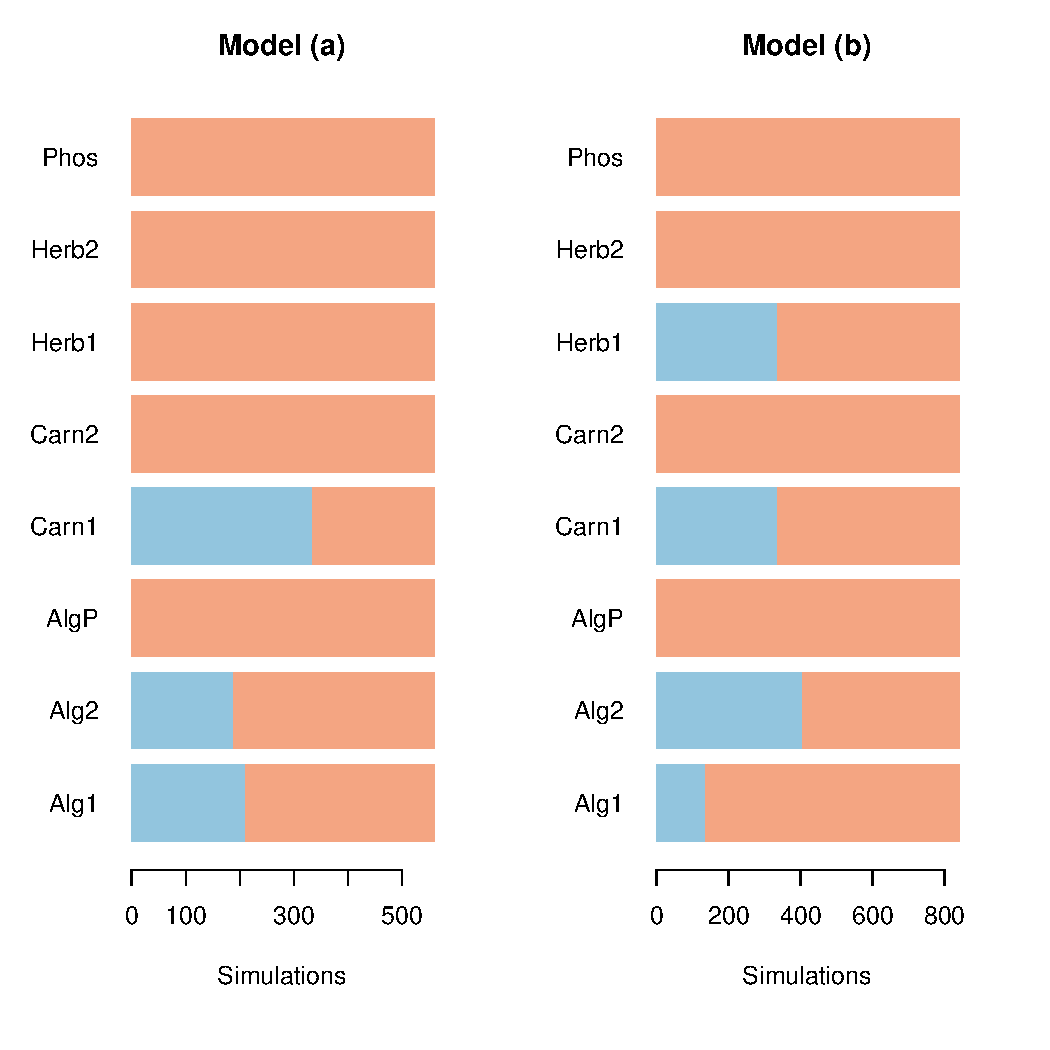
\includegraphics[width=\maxwidth]{figure/unnamed-chunk-3-1} 

\end{knitrout}
\caption{Simulation outcomes from the two lake mesocosm models in response to a
  positive press perturbation to phosphorous. Each plot shows the fraction of
  positive (orange), and negative (blue) outcomes at each node. The x-axis
  indicates the number of simulations (out of 1000 total) that match with the
  selection for `Monitor' shown in Figure~\ref{fig:Selector1}.}
  \label{fig:Perturb1}
\end{figure}

Approximately 50\% of the simulations match with observations for model (a),
whereas for model (b) this increases to over 80\%. This suggests that model (b)
provides a more parsimonious representation of the lake mesocosm system.
\cite{JMT2012} provide a direct comparison of the two models using Bayes factors.

\section{Example II: Antarctic mesocosm}
This example is based on experiments conducted at Australia's Davis Station in
Antarctica, which assessed the responses of a natural community of Antarctic
marine microbes from near-shore waters to elevated concentrations of $\mathrm{CO}_{2}$
using environmentally controlled tanks (mesocosms). Davidson et al.
(in prep) describe the main components of the Southern Ocean microbial loop
represented in these mesocosms and the ecological interactions between them.
Specifically:
\begin{itemize}
\item Small and large phytoplankton cells consume macronutrients and iron (Fe),
although iron is potentially less important for growth of small phytoplankton;
\item Small phytoplankton are consumed by heterotrophic nanoflagellates and
microzooplankton;
\item Large phytoplankton (diatoms) are consumed by microzooplankton;
\item Bacteria break down DOC (dissolved organic carbon) and are consumed by
heterotrophic nanoflagellates;
\item Phytoplankton, microzooplankton and heterotrophic nanoflagellates supply
the DOC pool.
\end{itemize}
These interactions are represented in a model that was built using Dia
(black-coloured edges in Figure~\ref{fig:Antarctic-a}).

When this system was subjected to elevated $\mathrm{CO}_{2}$ concentrations in experimental
mesocosms, the following responses were observed:
\begin{itemize}
\item Small phytoplankton increased;
\item Large phytoplankton decreased;
\item Heterotrophic nanoflagellates decreased; and
\item Bacteria increased.
\end{itemize}

In the model shown in Figure~\ref{fig:Antarctic-a} we assume that the direct
effects of $\mathrm{CO}_{2}$ correspond with these observed changes.
\vspace{1cm}

\begin{figure}[ht]
  \centering
  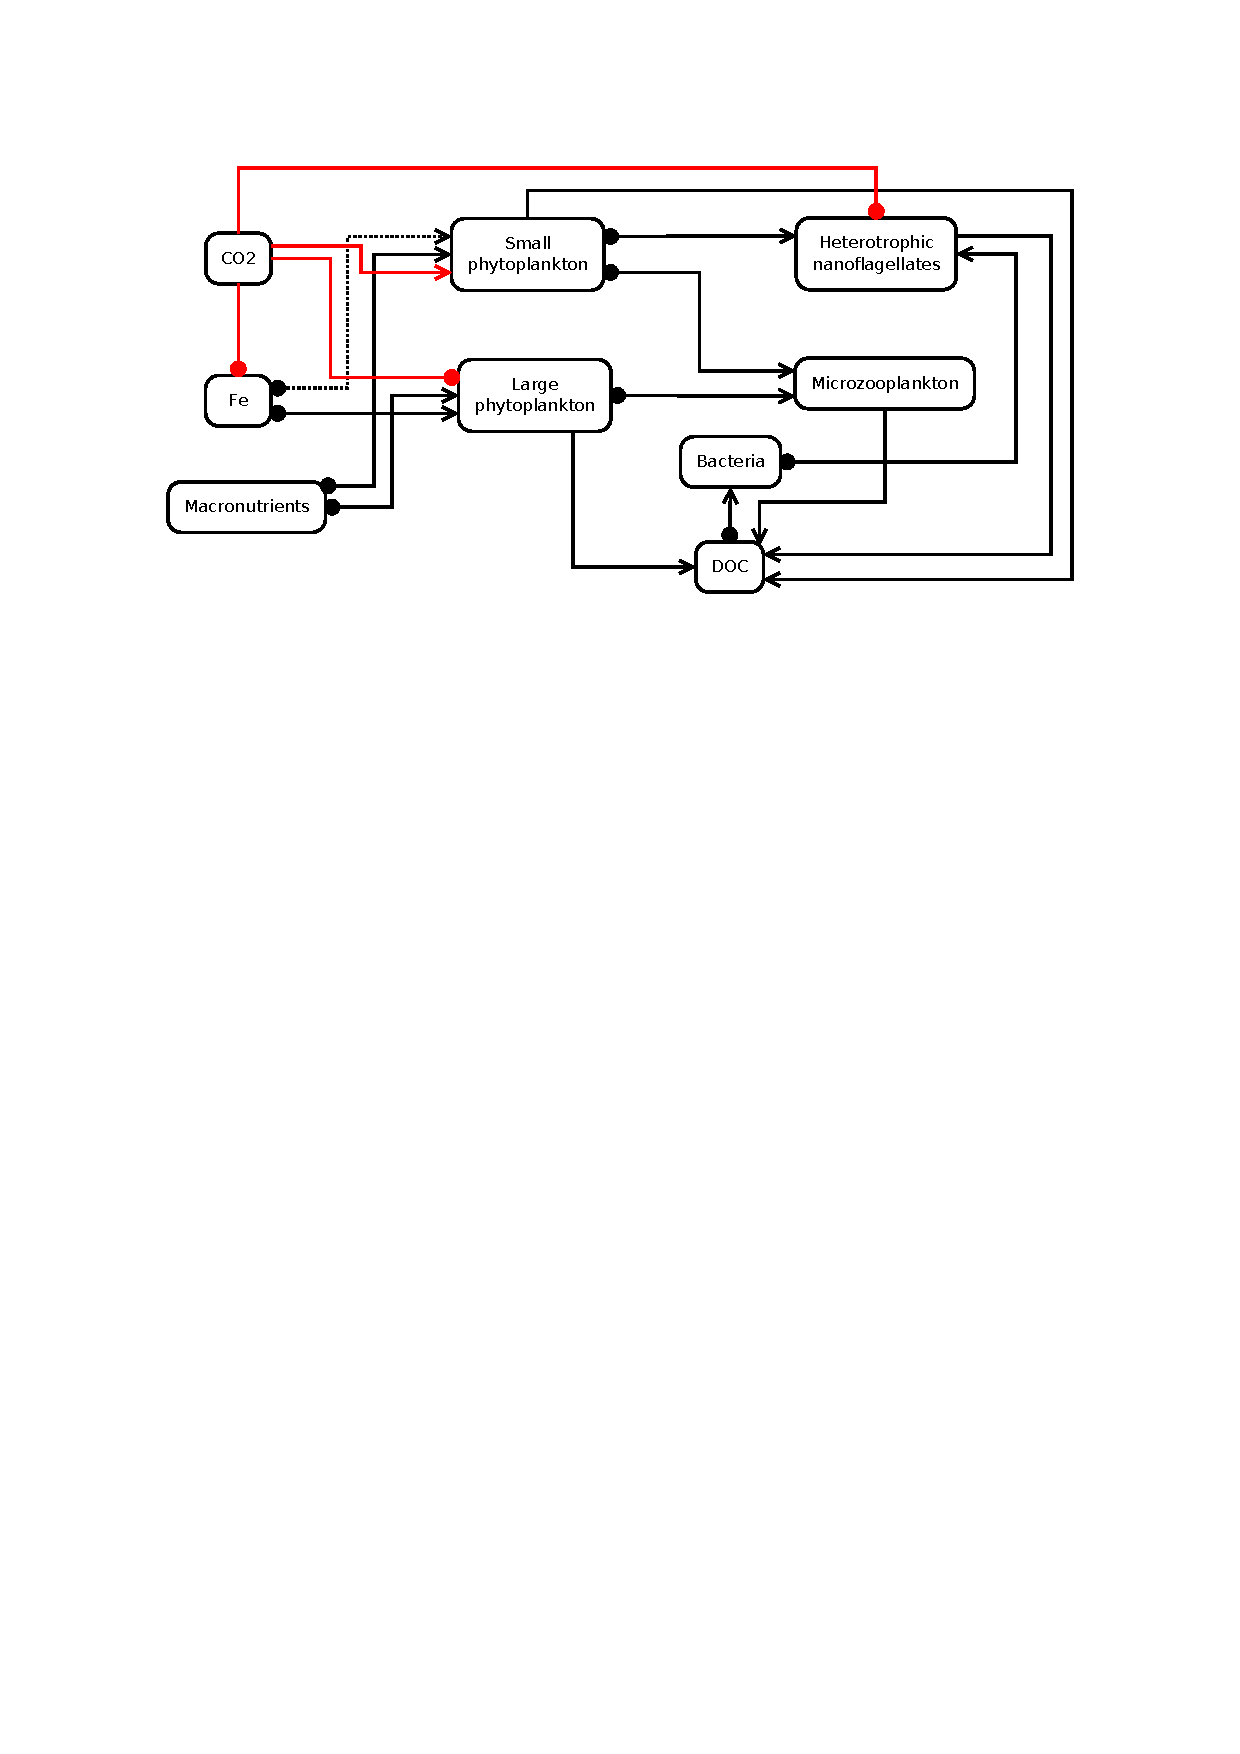
\includegraphics{Antarctic-a.pdf}
  \caption{Model (a) representing the effects of $\mathrm{CO}_{2}$ on the Southern Ocean
  microbial loop, determined directly from observed responses in experimental
  mesocosms. These direct effects are shown in red.}
  \label{fig:Antarctic-a}
\end{figure}
\vspace{1cm}

We then analyse the response this model to a positive press perturbation to
$\mathrm{CO}_{2}$. In this case we enforce a specific ordering of the nodes, and also
enforce self-limitation for each model variable.
\begin{knitrout}
\definecolor{shadecolor}{rgb}{0.969, 0.969, 0.969}\color{fgcolor}\begin{kframe}
\begin{alltt}
\hlcom{## Enforce the ordering of nodes.}
\hlstd{labels} \hlkwb{<-} \hlkwd{c}\hlstd{(}\hlstr{"CO2"}\hlstd{,}\hlstr{"Fe"}\hlstd{,}\hlstr{"Macronutrients"}\hlstd{,}\hlstr{"Small phytoplankton"}\hlstd{,}
            \hlstr{"Large phytoplankton"}\hlstd{,}\hlstr{"Heterotrophic nanoflagellates"}\hlstd{,}
            \hlstr{"Microzooplankton"}\hlstd{,}\hlstr{"Bacteria"}\hlstd{,}\hlstr{"DOC"}\hlstd{)}
\hlstd{antarctic.a} \hlkwb{<-} \hlkwd{model.dia}\hlstd{(}\hlstr{"Antarctic-a.dia"}\hlstd{,}\hlkwc{labels}\hlstd{=labels)}
\hlstd{antarctic.a} \hlkwb{<-} \hlkwd{enforce.limitation}\hlstd{(antarctic.a)}
\end{alltt}
\end{kframe}
\end{knitrout}
As for Example I, we then simulate and use \texttt{impact.barplot} (with
the selections shown in Figure~\ref{fig:Selector2}) to produce
Figure~\ref{fig:Perturb2}.
@
\begin{knitrout}
\definecolor{shadecolor}{rgb}{0.969, 0.969, 0.969}\color{fgcolor}\begin{kframe}
\begin{alltt}
\hlstd{simantarctic.a} \hlkwb{<-} \hlkwd{system.simulate}\hlstd{(}\hlnum{1000}\hlstd{,antarctic.a)}
\hlkwd{impact.barplot}\hlstd{(simantarctic.a)}
\end{alltt}
\end{kframe}
\end{knitrout}

\begin{figure}[ht]
  \centering
  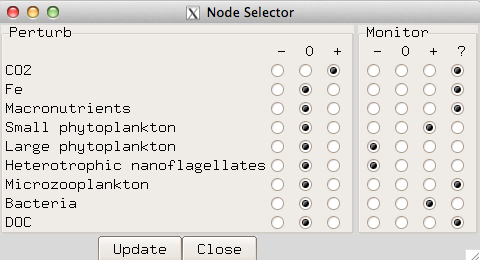
\includegraphics[width=0.6\textwidth]{Antarctic-selector.png}
  \caption{Node selector for the Antarctic mesocosm example.}
  \label{fig:Selector2}
\end{figure}

\begin{figure}[ht]
  \centering
\begin{knitrout}
\definecolor{shadecolor}{rgb}{0.969, 0.969, 0.969}\color{fgcolor}
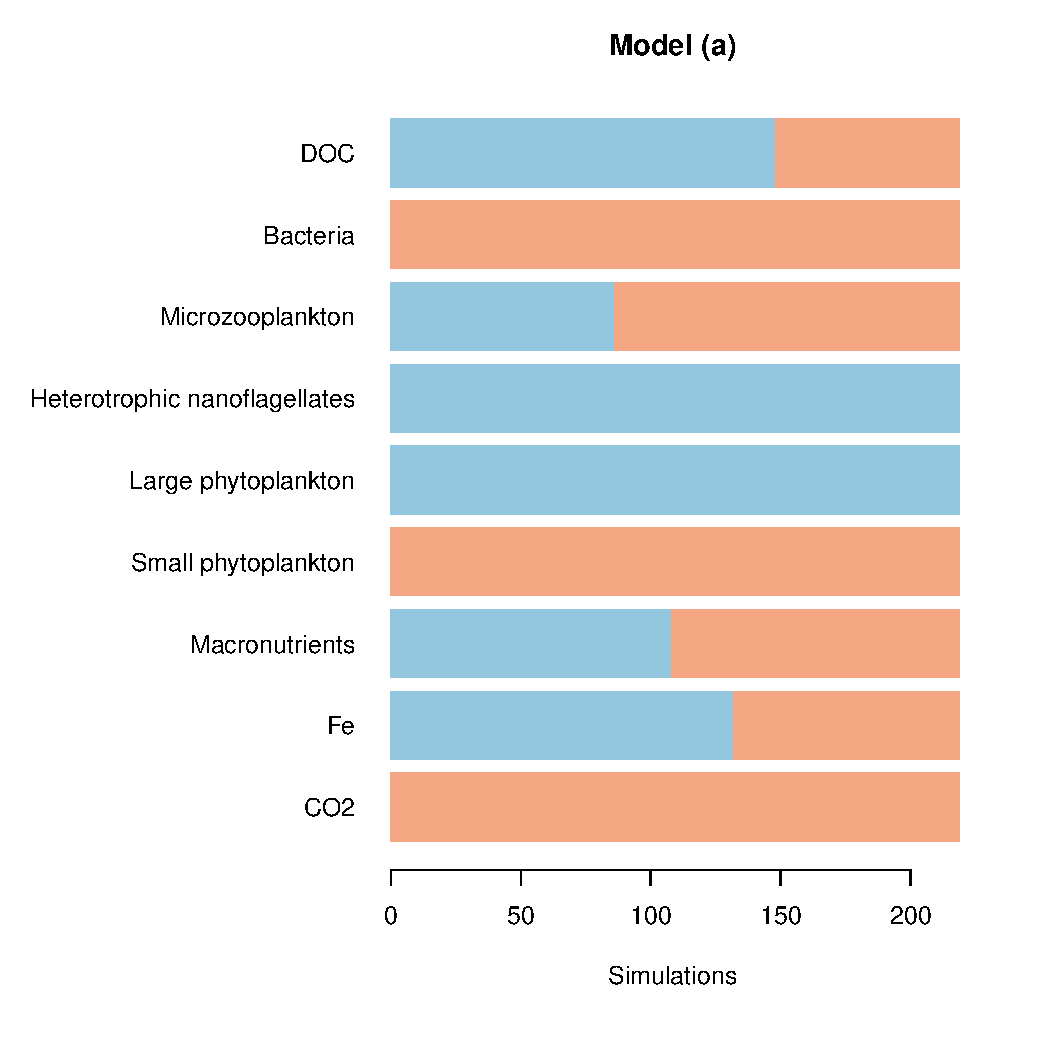
\includegraphics[width=\maxwidth]{figure/unnamed-chunk-6-1} 

\end{knitrout}
\caption{Simulation outcomes in response to a positive press perturbation to
  $\mathrm{CO}_{2}$ for Antarctic mesocosm model (a). Each plot shows the fraction of
  positive (orange), and negative (blue) outcomes at each node.}
  \label{fig:Perturb2}
\end{figure}
\clearpage

For this version of the model, less than 20\% of the simulations match with our
`Monitor' criteria, suggesting that it does not provide a particularly good
representation of the Antarctic microbial loop system or its response to
increased $\mathrm{CO}_{2}$ concentrations. Given that increases in
dissolved $\mathrm{CO}_{2}$ are generally expected to have negative impacts of the growth
of marine organisms, we could assume a direct negative effect of $\mathrm{CO}_{2}$ on each
of large phytoplankton, small phytoplankton, heterotrophic nanoflagellates, and
also the pool of available iron (Figure~\ref{fig:Antarctic-b}).
\vspace{1cm}

\begin{figure}[ht]
  \centering
  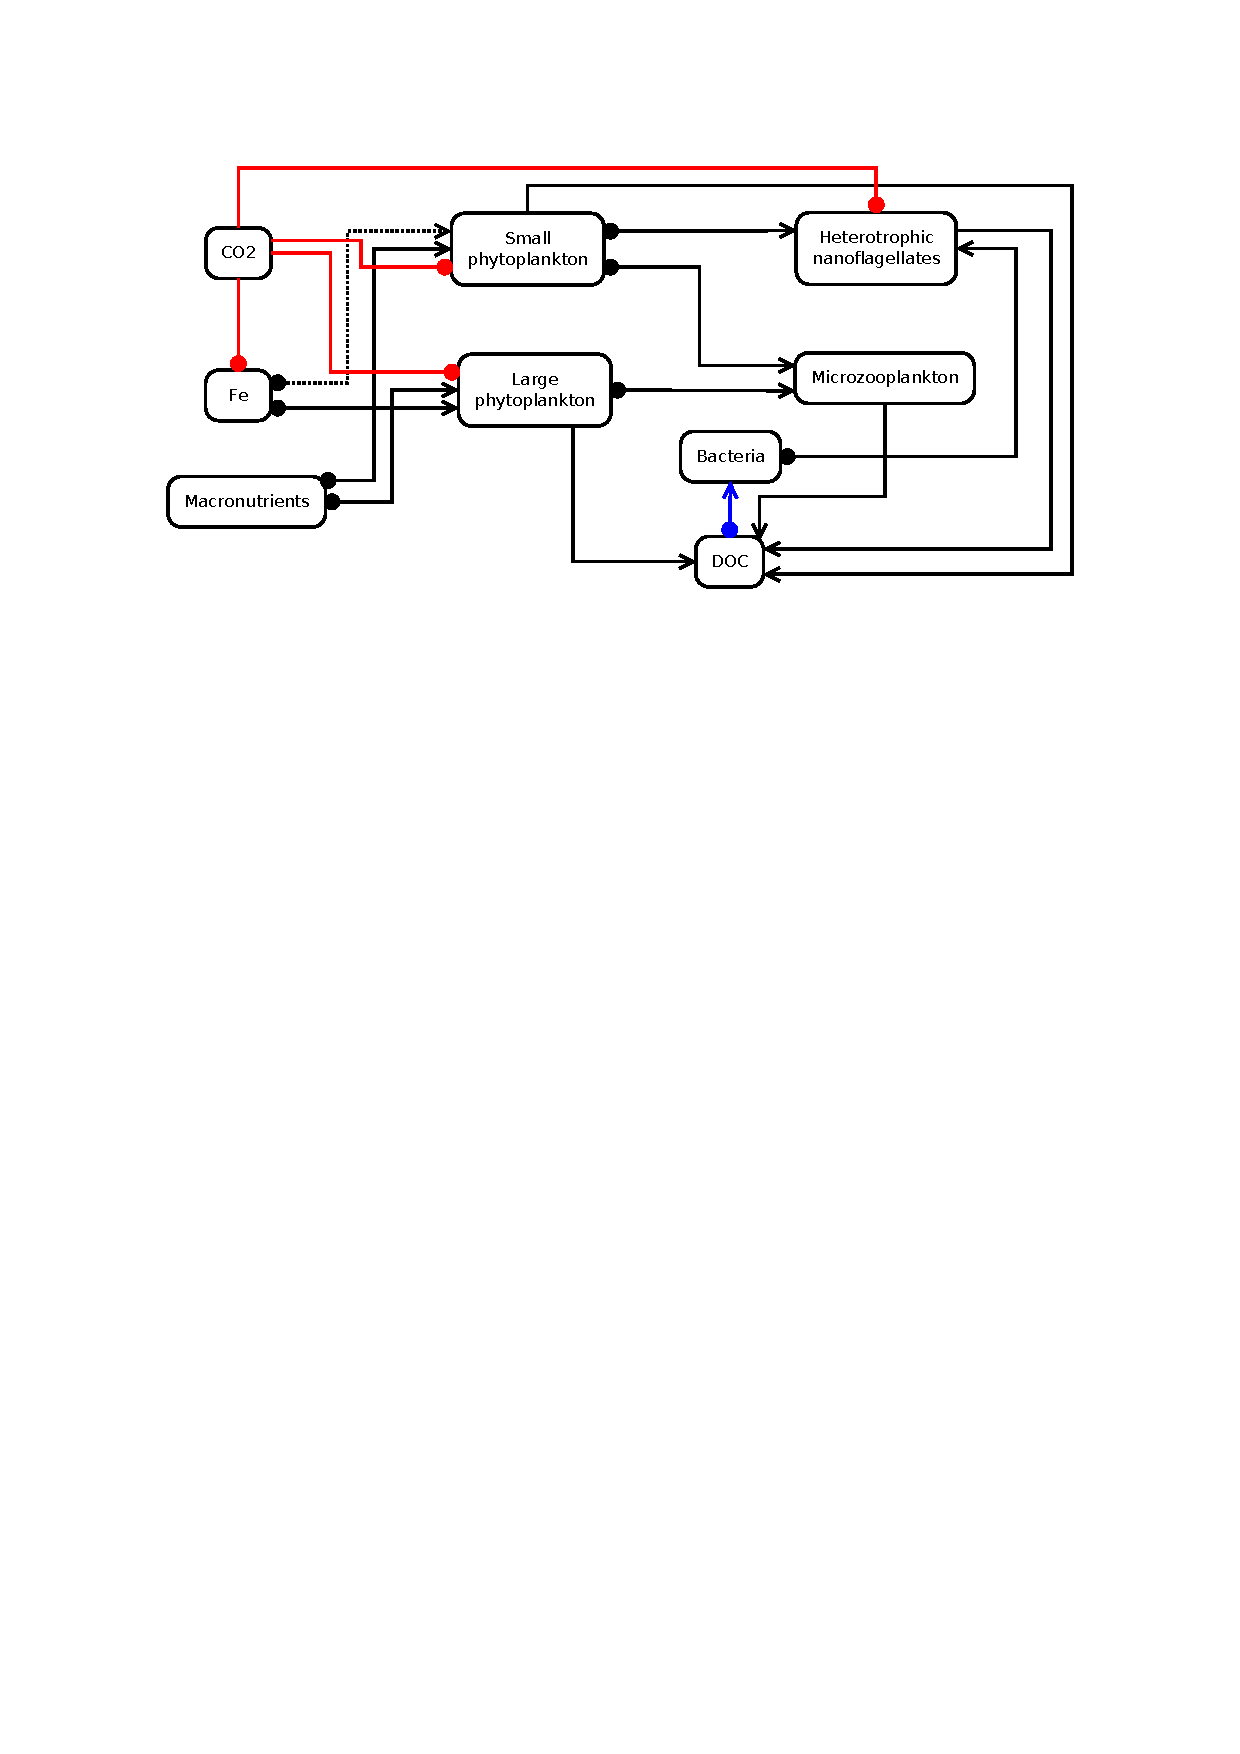
\includegraphics{Antarctic-b.pdf}
  \caption{Alternative model (b) representing the effects of $\mathrm{CO}_{2}$ on the
  Southern  Ocean microbial loop.}
  \label{fig:Antarctic-b}
\end{figure}
\vspace{1cm}

Reading this alternative representation from a Dia file
\begin{knitrout}
\definecolor{shadecolor}{rgb}{0.969, 0.969, 0.969}\color{fgcolor}\begin{kframe}
\begin{alltt}
\hlstd{antarctic.b} \hlkwb{<-} \hlkwd{model.dia}\hlstd{(}\hlstr{"Antarctic-b.dia"}\hlstd{,}\hlkwc{labels}\hlstd{=labels)}
\hlstd{antarctic.b} \hlkwb{<-} \hlkwd{enforce.limitation}\hlstd{(antarctic.b)}
\end{alltt}
\end{kframe}
\end{knitrout}
and exploring simulation outcomes with \texttt{impact.barplot} (with the same
`Monitor' criteria as before) produces Figure~\ref{fig:Perturb3}.
@
\begin{knitrout}
\definecolor{shadecolor}{rgb}{0.969, 0.969, 0.969}\color{fgcolor}\begin{kframe}
\begin{alltt}
\hlstd{simantarctic.b} \hlkwb{<-} \hlkwd{system.simulate}\hlstd{(}\hlnum{1000}\hlstd{,antarctic.b)}
\hlkwd{impact.barplot}\hlstd{(simantarctic.b)}
\end{alltt}
\end{kframe}
\end{knitrout}

In this case, we still only see approximately 20\% of simulations that meet our
criteria, suggesting that we need to re-think the structure of our model.
Davidson et al. (in prep) indicate that bacteria ``transform dissolved organic
carbon (DOC)... thereby repackaging carbon and making it available to higher
trophic levels''. Looking at our original model, we haven't quite captured this
in our representation of interactions between bacteria, DOC and macronutrients.
In a third version of our microbial loop model (model (c) --
Figure~\ref{fig:Antarctic-c}) we therefore assume a negative effect of bacteria
on DOC and a positive effect of bacteria on macronutrients (which includes carbon).

Reading a third Dia version of the model
\begin{knitrout}
\definecolor{shadecolor}{rgb}{0.969, 0.969, 0.969}\color{fgcolor}\begin{kframe}
\begin{alltt}
\hlstd{antarctic.c} \hlkwb{<-} \hlkwd{model.dia}\hlstd{(}\hlstr{"Antarctic-c.dia"}\hlstd{,}\hlkwc{labels}\hlstd{=labels)}
\hlstd{antarctic.c} \hlkwb{<-} \hlkwd{enforce.limitation}\hlstd{(antarctic.c)}
\end{alltt}
\end{kframe}
\end{knitrout}
and repeating the simulation and \texttt{impact.barplot} steps from above gives
Figure~\ref{fig:Perturb4}.

\begin{figure}[ht]
  \centering
\begin{knitrout}
\definecolor{shadecolor}{rgb}{0.969, 0.969, 0.969}\color{fgcolor}
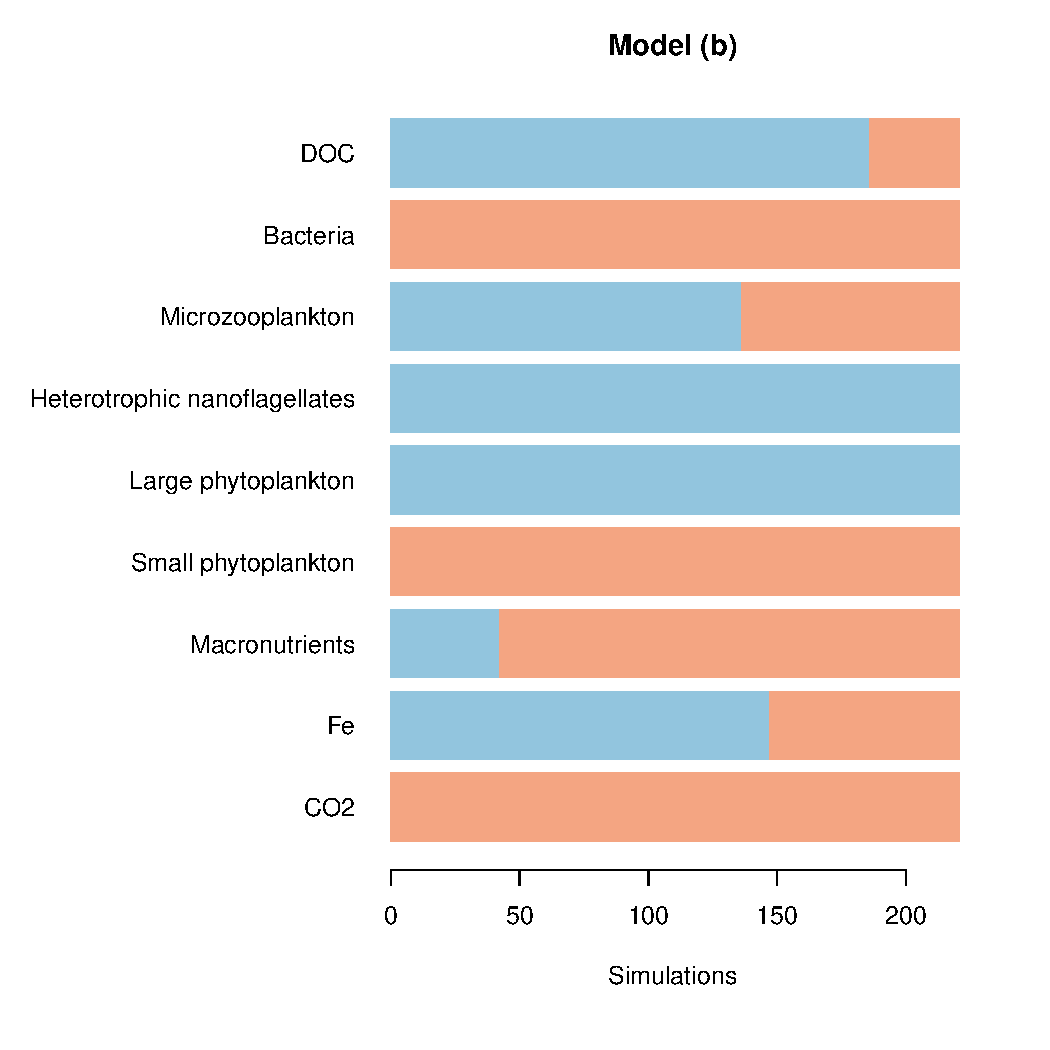
\includegraphics[width=\maxwidth]{figure/unnamed-chunk-10-1} 

\end{knitrout}
\caption{Simulation outcomes in response to a positive press perturbation to the
  $\mathrm{CO}_{2}$ for the alternative microbial loop model (b) shown in
  Figure~\ref{fig:Antarctic-b}.}
  \label{fig:Perturb3}
\end{figure}

\begin{figure}[ht]
  \centering
  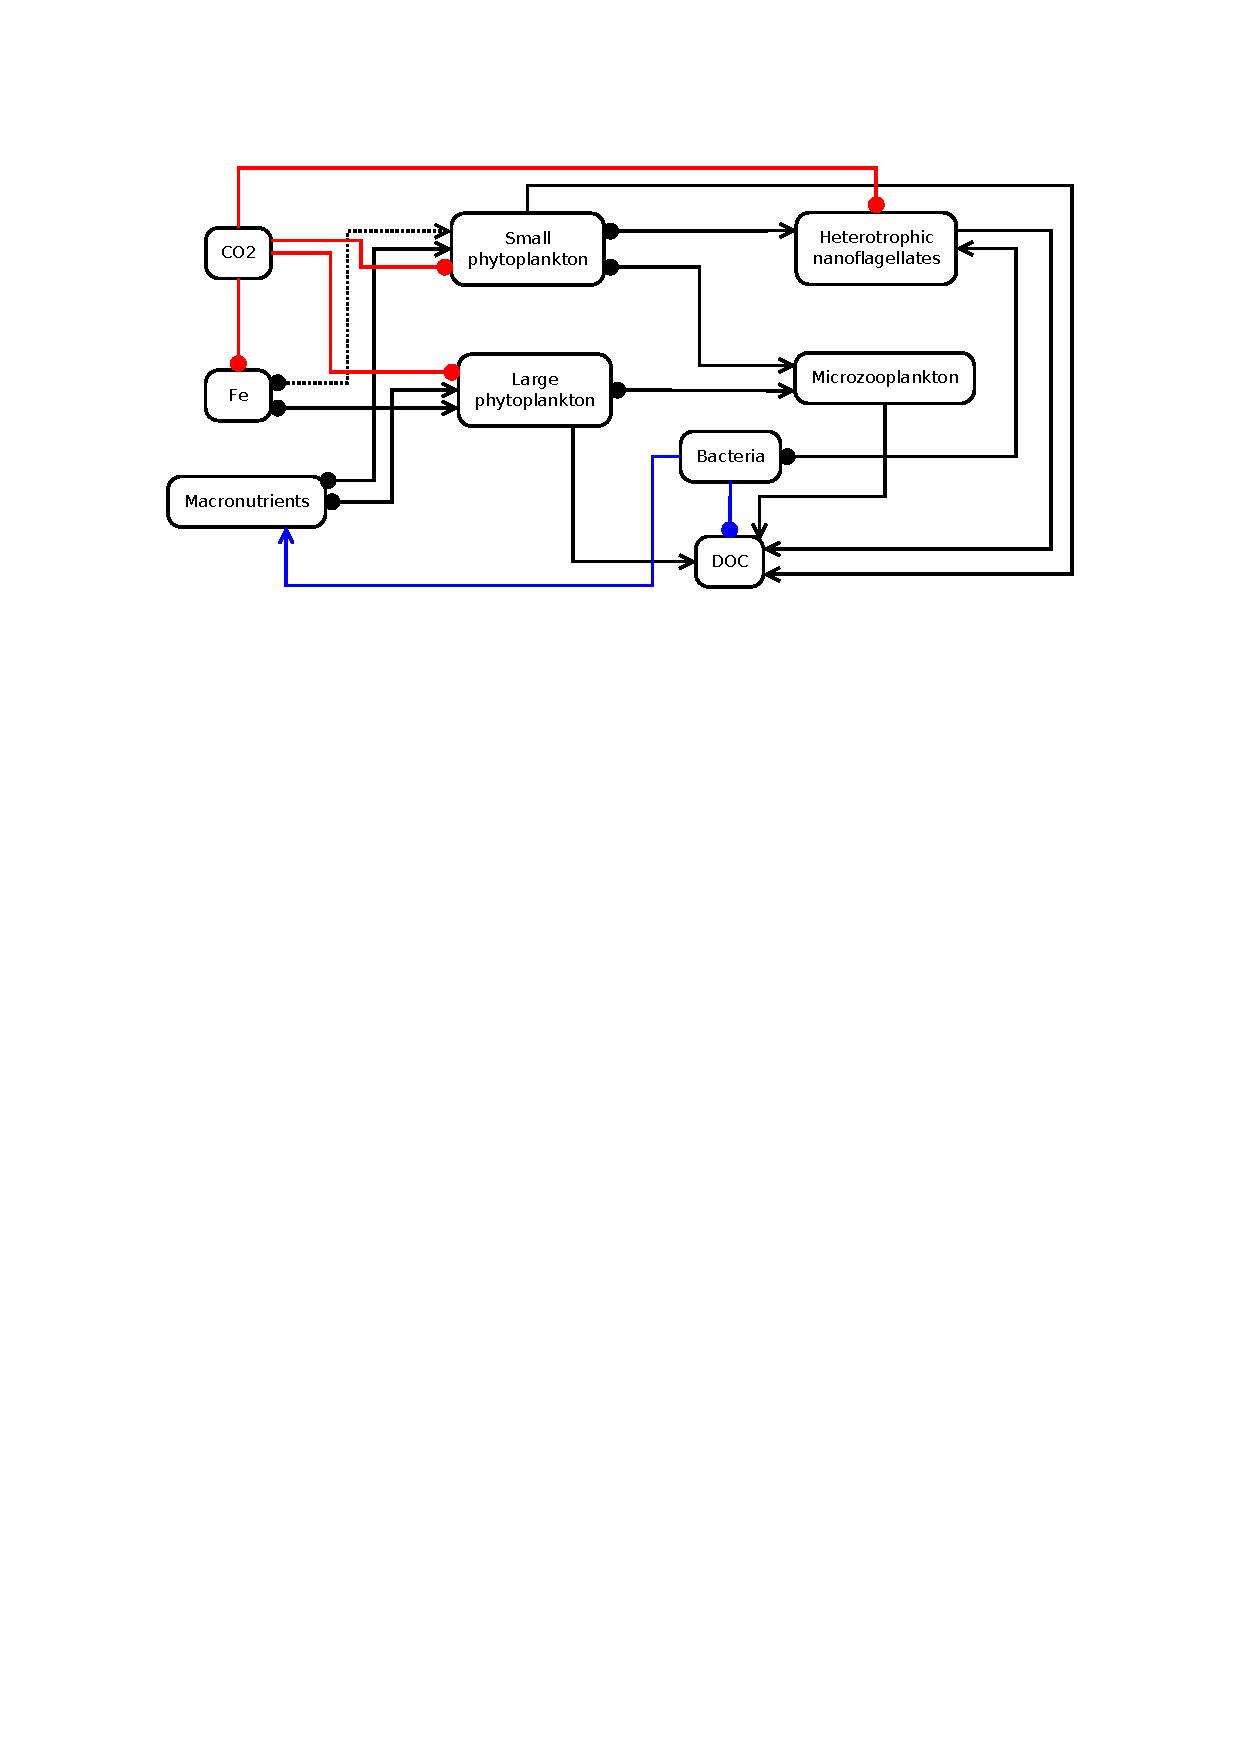
\includegraphics{Antarctic-c.pdf}
  \caption{Alternative model (c) representing the effects of $\mathrm{CO}_{2}$ on the
  Southern Ocean  microbial loop.}
  \label{fig:Antarctic-c}
\end{figure}

\begin{figure}[ht]
  \centering
\begin{knitrout}
\definecolor{shadecolor}{rgb}{0.969, 0.969, 0.969}\color{fgcolor}
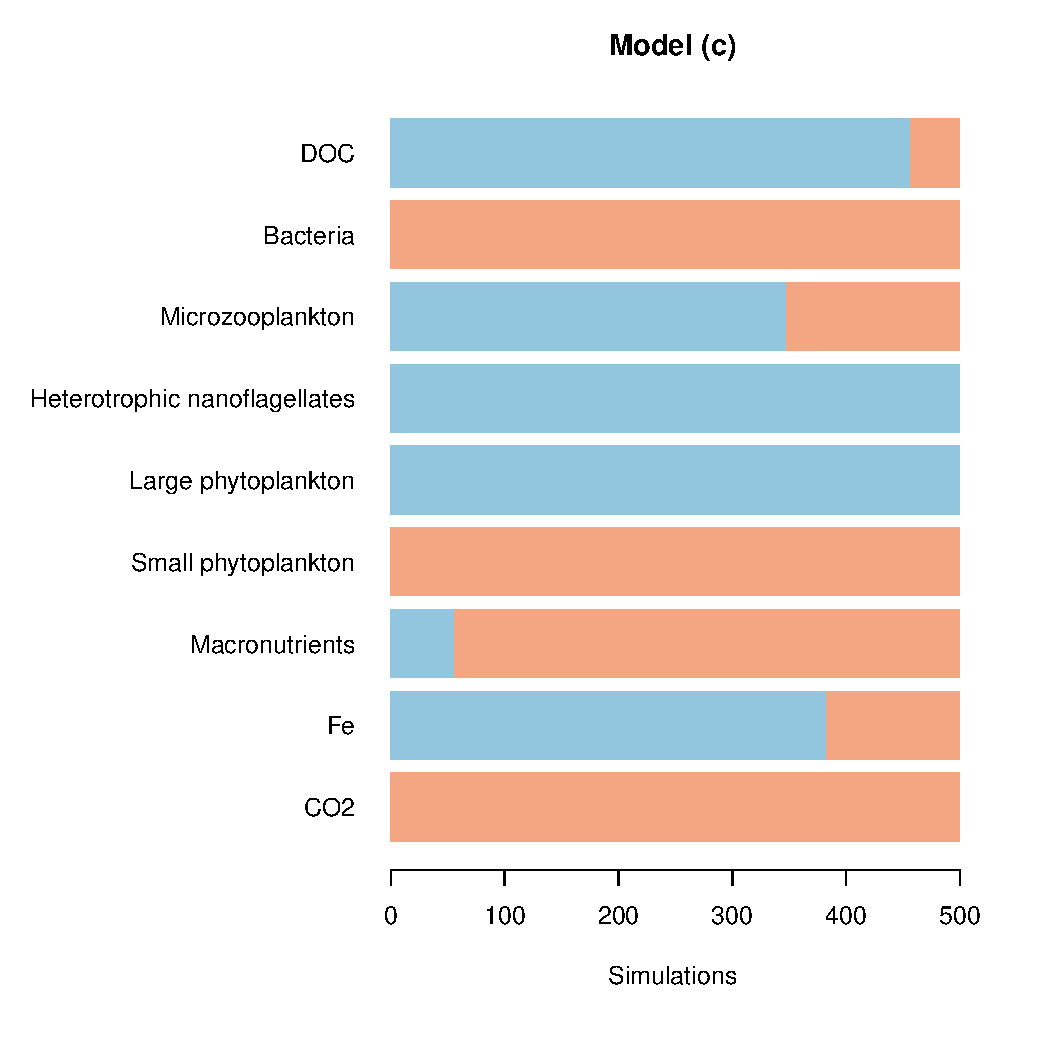
\includegraphics[width=\maxwidth]{figure/unnamed-chunk-11-1} 

\end{knitrout}
\caption{Simulation outcomes in response to a positive press perturbation to the
  $\mathrm{CO}_{2}$ for the alternative microbial loop model (c) shown in
  Figure~\ref{fig:Antarctic-c}.}
  \label{fig:Perturb4}
\end{figure}
\clearpage

\bibliographystyle{apalike}
\bibliography{QPress}

\end{document}
